\documentclass{standalone}
\usepackage{tikz}
\usetikzlibrary{patterns, positioning}
\usepackage[sfdefault]{ClearSans} %% option 'sfdefault' activates Clear Sans as the default text font
\usepackage[T1]{fontenc}

\begin{document}
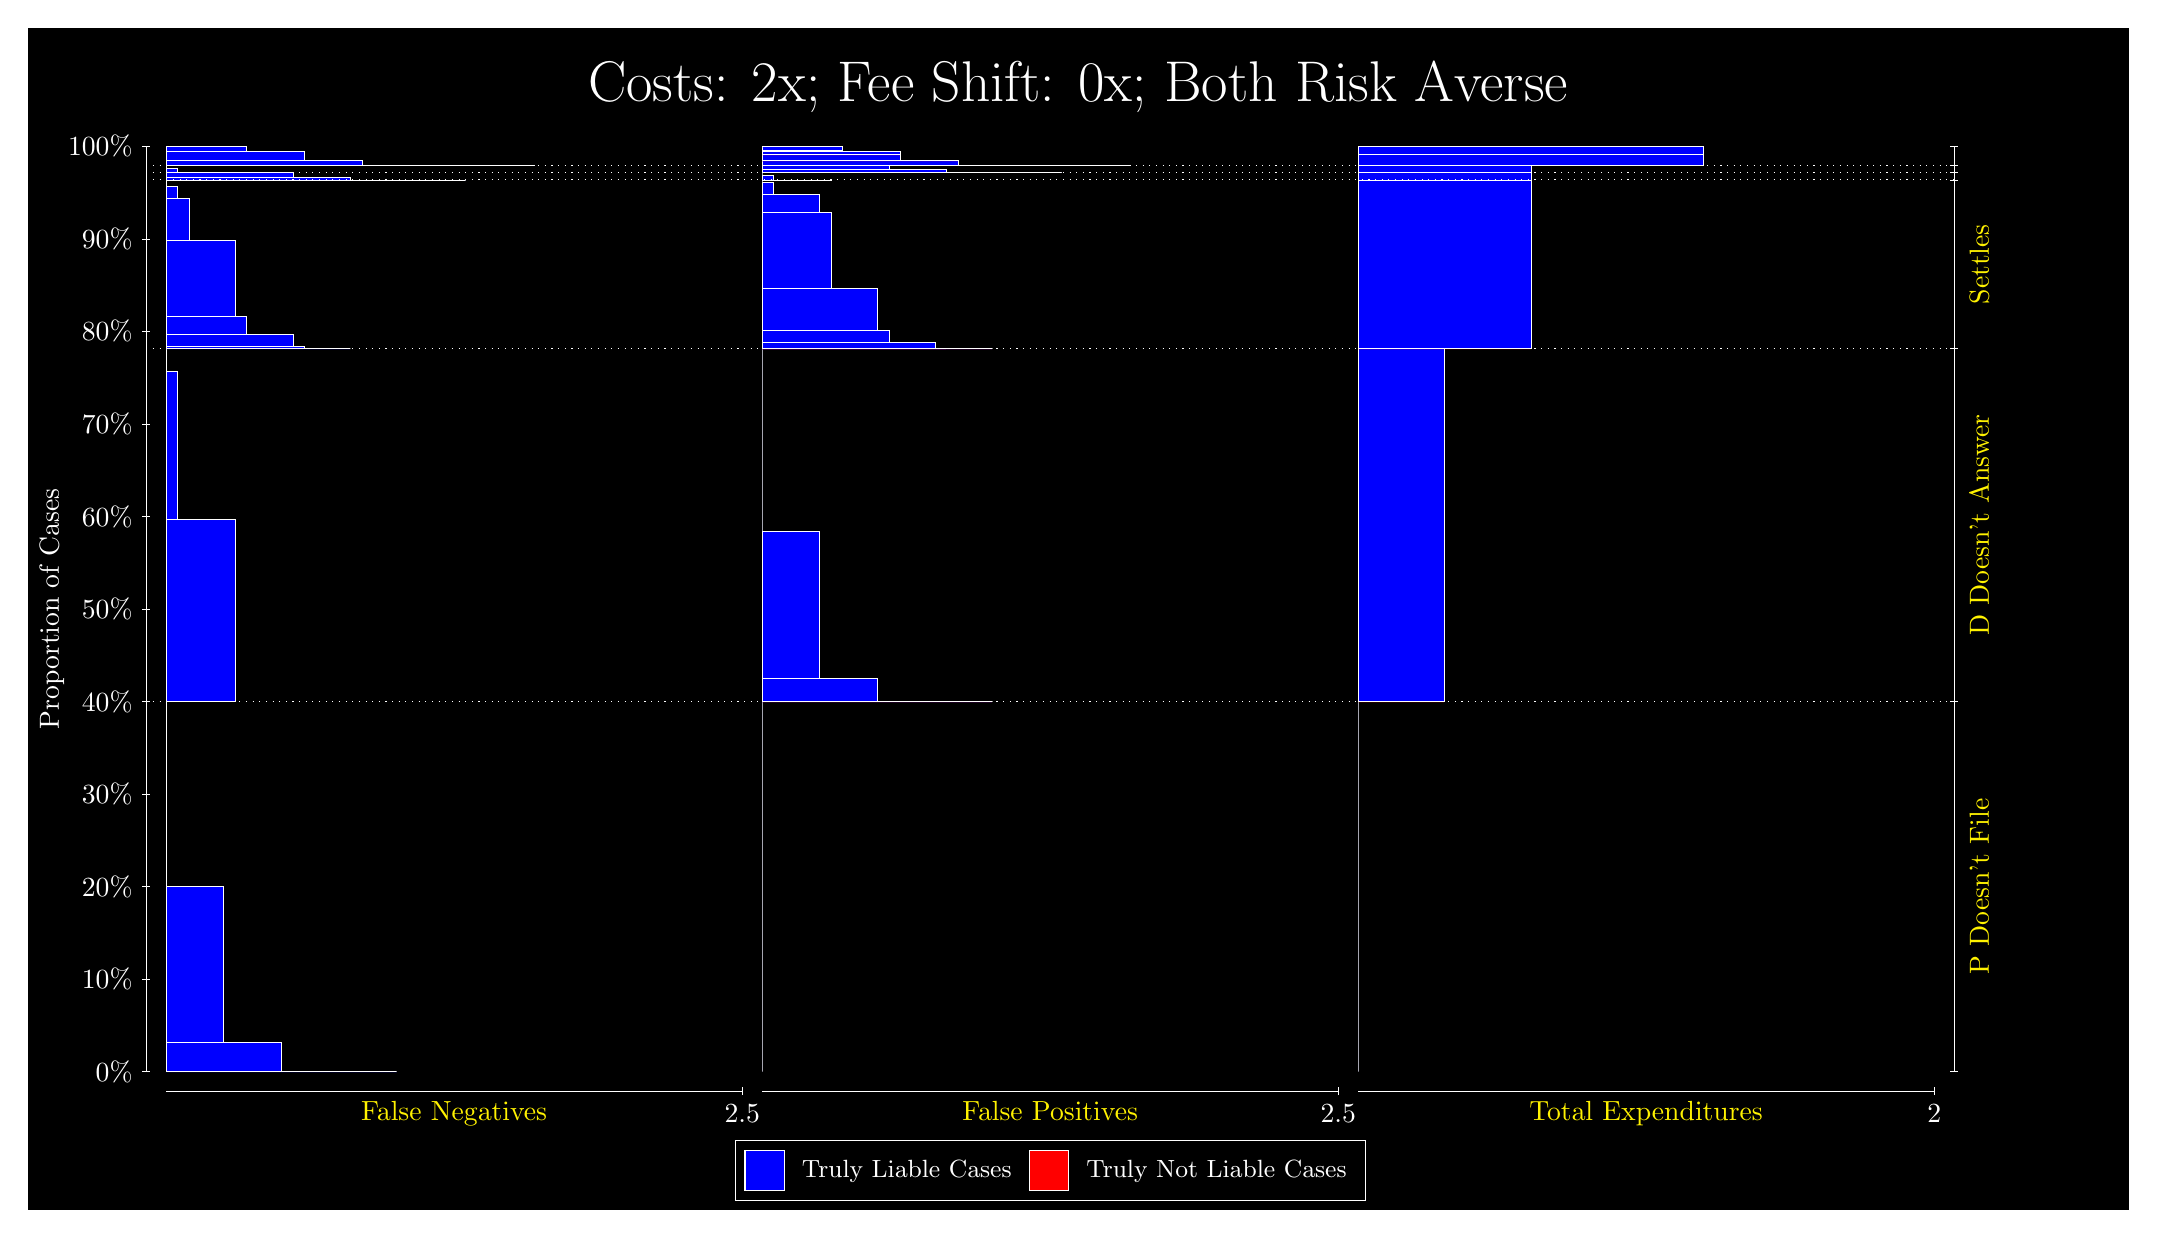
\begin{tikzpicture}
\draw[fill=black] (0,0) rectangle (26.667,15);
\draw[text=white] (0,13.5) rectangle (26.667,15) node[midway] {\huge Costs: 2x; Fee Shift: 0x; Both Risk Averse};
\draw[white, very thin] (1.5,1.75) -- (1.5,13.5);
\node[rotate=90, text=white, anchor=center] at (0.3, 7.625) {Proportion of Cases};
\draw[white, very thin] (1.45,1.75) -- (1.55,1.75);
\node[text=white, anchor=east] at (1.45, 1.75) {0\%};
\draw[white, very thin] (1.45,2.925) -- (1.55,2.925);
\node[text=white, anchor=east] at (1.45, 2.925) {10\%};
\draw[white, very thin] (1.45,4.1) -- (1.55,4.1);
\node[text=white, anchor=east] at (1.45, 4.1) {20\%};
\draw[white, very thin] (1.45,5.275) -- (1.55,5.275);
\node[text=white, anchor=east] at (1.45, 5.275) {30\%};
\draw[white, very thin] (1.45,6.45) -- (1.55,6.45);
\node[text=white, anchor=east] at (1.45, 6.45) {40\%};
\draw[white, very thin] (1.45,7.625) -- (1.55,7.625);
\node[text=white, anchor=east] at (1.45, 7.625) {50\%};
\draw[white, very thin] (1.45,8.8) -- (1.55,8.8);
\node[text=white, anchor=east] at (1.45, 8.8) {60\%};
\draw[white, very thin] (1.45,9.975) -- (1.55,9.975);
\node[text=white, anchor=east] at (1.45, 9.975) {70\%};
\draw[white, very thin] (1.45,11.15) -- (1.55,11.15);
\node[text=white, anchor=east] at (1.45, 11.15) {80\%};
\draw[white, very thin] (1.45,12.325) -- (1.55,12.325);
\node[text=white, anchor=east] at (1.45, 12.325) {90\%};
\draw[white, very thin] (1.45,13.5) -- (1.55,13.5);
\node[text=white, anchor=east] at (1.45, 13.5) {100\%};

\draw[white, very thin] (24.457,1.75) -- (24.457,13.5);
\draw[white, very thin] (24.407,1.75) -- (24.507,1.75);
\node[anchor=west] at (24.407, 1.75) {};
\draw[white, very thin] (24.407,6.4489) -- (24.507,6.4489);
\node[anchor=west] at (24.407, 6.4489) {};
\draw[white, very thin] (24.407,10.931) -- (24.507,10.931);
\node[anchor=west] at (24.407, 10.931) {};
\draw[white, very thin] (24.407,13.073) -- (24.507,13.073);
\node[anchor=west] at (24.407, 13.073) {};
\draw[white, very thin] (24.407,13.17) -- (24.507,13.17);
\node[anchor=west] at (24.407, 13.17) {};
\draw[white, very thin] (24.407,13.257) -- (24.507,13.257);
\node[anchor=west] at (24.407, 13.257) {};
\draw[white, very thin] (24.407,13.5) -- (24.507,13.5);
\node[anchor=west] at (24.407, 13.5) {};

\draw[white, very thin, fill=blue] (1.75,1.75) rectangle (4.6775,1.75);
\draw[white, very thin, fill=blue] (1.75,1.75) rectangle (3.9457,1.7532);
\draw[white, very thin, fill=blue] (1.75,1.7532) rectangle (3.2138,2.126);
\draw[white, very thin, fill=blue] (1.75,2.126) rectangle (2.4819,4.1027);
\draw[white, very thin, fill=red] (1.75,4.1027) rectangle (1.75,4.1027);
\draw[white, very thin, fill=blue] (1.75,4.1027) rectangle (1.75,6.4489);
\draw[white, very thin, fill=blue] (1.75,6.4489) rectangle (2.6283,8.7667);
\draw[white, very thin, fill=blue] (1.75,8.7667) rectangle (1.8964,10.637);
\draw[white, very thin, fill=red] (1.75,10.637) rectangle (1.75,10.637);
\draw[white, very thin, fill=blue] (1.75,10.637) rectangle (1.75,10.931);
\draw[white, very thin, fill=blue] (1.75,10.931) rectangle (4.092,10.931);
\draw[white, very thin, fill=blue] (1.75,10.931) rectangle (3.5065,10.961);
\draw[white, very thin, fill=blue] (1.75,10.961) rectangle (3.3602,11.112);
\draw[white, very thin, fill=blue] (1.75,11.112) rectangle (2.7746,11.339);
\draw[white, very thin, fill=blue] (1.75,11.339) rectangle (2.6283,12.308);
\draw[white, very thin, fill=blue] (1.75,12.308) rectangle (2.0428,12.846);
\draw[white, very thin, fill=blue] (1.75,12.846) rectangle (1.8964,12.997);
\draw[white, very thin, fill=red] (1.75,12.997) rectangle (1.75,12.997);
\draw[white, very thin, fill=blue] (1.75,12.997) rectangle (1.75,13.073);
\draw[white, very thin, fill=blue] (1.75,13.073) rectangle (5.5558,13.073);
\draw[white, very thin, fill=blue] (1.75,13.073) rectangle (4.8239,13.073);
\draw[white, very thin, fill=blue] (1.75,13.073) rectangle (4.092,13.109);
\draw[white, very thin, fill=blue] (1.75,13.109) rectangle (3.3602,13.169);
\draw[white, very thin, fill=blue] (1.75,13.169) rectangle (2.6283,13.17);
\draw[white, very thin, fill=red] (1.75,13.17) rectangle (1.75,13.17);
\draw[white, very thin, fill=blue] (1.75,13.17) rectangle (2.6283,13.172);
\draw[white, very thin, fill=blue] (1.75,13.172) rectangle (1.8964,13.225);
\draw[white, very thin, fill=red] (1.75,13.225) rectangle (1.75,13.225);
\draw[white, very thin, fill=blue] (1.75,13.225) rectangle (1.75,13.257);
\draw[white, very thin, fill=blue] (1.75,13.257) rectangle (6.4341,13.257);
\draw[white, very thin, fill=blue] (1.75,13.257) rectangle (5.7022,13.257);
\draw[white, very thin, fill=blue] (1.75,13.257) rectangle (4.9703,13.261);
\draw[white, very thin, fill=blue] (1.75,13.261) rectangle (4.2384,13.317);
\draw[white, very thin, fill=blue] (1.75,13.317) rectangle (3.5065,13.439);
\draw[white, very thin, fill=blue] (1.75,13.439) rectangle (2.7746,13.496);
\draw[white, very thin, fill=blue] (1.75,13.496) rectangle (2.0428,13.5);
\draw[white, very thin, fill=red] (1.75,13.5) rectangle (1.75,13.5);
\draw[white, very thin, fill=blue] (1.75,13.5) rectangle (1.75,13.5);
\draw[white, very thin, fill=red] (9.3189,1.75) rectangle (9.3189,1.75);
\draw[white, very thin, fill=blue] (9.3189,1.75) rectangle (9.3189,6.4489);
\draw[white, very thin, fill=red] (9.3189,6.4489) rectangle (12.246,6.4489);
\draw[white, very thin, fill=blue] (9.3189,6.4489) rectangle (12.246,6.4489);
\draw[white, very thin, fill=blue] (9.3189,6.4489) rectangle (11.515,6.4494);
\draw[white, very thin, fill=blue] (9.3189,6.4494) rectangle (10.783,6.743);
\draw[white, very thin, fill=blue] (9.3189,6.743) rectangle (10.051,8.6133);
\draw[white, very thin, fill=blue] (9.3189,8.6133) rectangle (9.3189,10.931);
\draw[white, very thin, fill=red] (9.3189,10.931) rectangle (12.246,10.931);
\draw[white, very thin, fill=blue] (9.3189,10.931) rectangle (12.246,10.931);
\draw[white, very thin, fill=red] (9.3189,10.931) rectangle (11.661,10.931);
\draw[white, very thin, fill=blue] (9.3189,10.931) rectangle (11.661,10.931);
\draw[white, very thin, fill=blue] (9.3189,10.931) rectangle (11.515,11.007);
\draw[white, very thin, fill=blue] (9.3189,11.007) rectangle (10.929,11.158);
\draw[white, very thin, fill=blue] (9.3189,11.158) rectangle (10.783,11.696);
\draw[white, very thin, fill=blue] (9.3189,11.696) rectangle (10.197,12.664);
\draw[white, very thin, fill=blue] (9.3189,12.664) rectangle (10.051,12.892);
\draw[white, very thin, fill=blue] (9.3189,12.892) rectangle (9.4652,13.043);
\draw[white, very thin, fill=blue] (9.3189,13.043) rectangle (9.3189,13.073);
\draw[white, very thin, fill=red] (9.3189,13.073) rectangle (10.197,13.073);
\draw[white, very thin, fill=blue] (9.3189,13.073) rectangle (10.197,13.074);
\draw[white, very thin, fill=blue] (9.3189,13.074) rectangle (9.4652,13.134);
\draw[white, very thin, fill=blue] (9.3189,13.134) rectangle (9.3189,13.17);
\draw[white, very thin, fill=red] (9.3189,13.17) rectangle (13.125,13.17);
\draw[white, very thin, fill=blue] (9.3189,13.17) rectangle (13.125,13.17);
\draw[white, very thin, fill=blue] (9.3189,13.17) rectangle (12.393,13.17);
\draw[white, very thin, fill=blue] (9.3189,13.17) rectangle (11.661,13.203);
\draw[white, very thin, fill=blue] (9.3189,13.203) rectangle (10.929,13.256);
\draw[white, very thin, fill=blue] (9.3189,13.256) rectangle (10.197,13.257);
\draw[white, very thin, fill=red] (9.3189,13.257) rectangle (14.003,13.257);
\draw[white, very thin, fill=blue] (9.3189,13.257) rectangle (14.003,13.257);
\draw[white, very thin, fill=red] (9.3189,13.257) rectangle (13.271,13.257);
\draw[white, very thin, fill=blue] (9.3189,13.257) rectangle (13.271,13.257);
\draw[white, very thin, fill=red] (9.3189,13.257) rectangle (12.539,13.257);
\draw[white, very thin, fill=blue] (9.3189,13.257) rectangle (12.539,13.262);
\draw[white, very thin, fill=blue] (9.3189,13.262) rectangle (11.807,13.318);
\draw[white, very thin, fill=red] (9.3189,13.318) rectangle (11.807,13.318);
\draw[white, very thin, fill=blue] (9.3189,13.318) rectangle (11.807,13.318);
\draw[white, very thin, fill=blue] (9.3189,13.318) rectangle (11.075,13.395);
\draw[white, very thin, fill=red] (9.3189,13.395) rectangle (11.075,13.395);
\draw[white, very thin, fill=blue] (9.3189,13.395) rectangle (11.075,13.44);
\draw[white, very thin, fill=blue] (9.3189,13.44) rectangle (10.344,13.451);
\draw[white, very thin, fill=blue] (9.3189,13.451) rectangle (10.344,13.497);
\draw[white, very thin, fill=blue] (9.3189,13.497) rectangle (9.6116,13.497);
\draw[white, very thin, fill=blue] (9.3189,13.497) rectangle (9.6116,13.5);
\draw[white, very thin, fill=blue] (9.3189,13.5) rectangle (9.3189,13.5);
\draw[white, very thin, fill=red] (16.888,1.75) rectangle (16.888,1.75);
\draw[white, very thin, fill=blue] (16.888,1.75) rectangle (16.888,6.4489);
\draw[white, very thin, fill=red] (16.888,6.4489) rectangle (17.986,6.4489);
\draw[white, very thin, fill=blue] (16.888,6.4489) rectangle (17.986,10.931);
\draw[white, very thin, fill=red] (16.888,10.931) rectangle (19.083,10.931);
\draw[white, very thin, fill=blue] (16.888,10.931) rectangle (19.083,13.073);
\draw[white, very thin, fill=red] (16.888,13.073) rectangle (19.083,13.073);
\draw[white, very thin, fill=blue] (16.888,13.073) rectangle (19.083,13.17);
\draw[white, very thin, fill=red] (16.888,13.17) rectangle (19.083,13.17);
\draw[white, very thin, fill=blue] (16.888,13.17) rectangle (19.083,13.257);
\draw[white, very thin, fill=red] (16.888,13.257) rectangle (21.279,13.257);
\draw[white, very thin, fill=blue] (16.888,13.257) rectangle (21.279,13.405);
\draw[white, very thin, fill=red] (16.888,13.405) rectangle (21.279,13.405);
\draw[white, very thin, fill=blue] (16.888,13.405) rectangle (21.279,13.5);
\draw[white, dotted] (1.5,6.4489) -- (24.457,6.4489);
\draw[white, dotted] (1.5,10.931) -- (24.457,10.931);
\draw[white, dotted] (1.5,13.073) -- (24.457,13.073);
\draw[white, dotted] (1.5,13.17) -- (24.457,13.17);
\draw[white, dotted] (1.5,13.257) -- (24.457,13.257);
\draw[white, very thin] (1.75,1.5) -- (9.0689,1.5);
\node[text=yellow, anchor=north] at (5.4094, 1.5) {False Negatives};
\draw[white, very thin] (9.0689,1.45) -- (9.0689,1.55);
\node[text=white, anchor=north] at (9.0689, 1.45) {2.5};

\draw[white, very thin] (9.3189,1.5) -- (16.638,1.5);
\node[text=yellow, anchor=north] at (12.978, 1.5) {False Positives};
\draw[white, very thin] (16.638,1.45) -- (16.638,1.55);
\node[text=white, anchor=north] at (16.638, 1.45) {2.5};

\draw[white, very thin] (16.888,1.5) -- (24.207,1.5);
\node[text=yellow, anchor=north] at (20.547, 1.5) {Total Expenditures};
\draw[white, very thin] (24.207,1.45) -- (24.207,1.55);
\node[text=white, anchor=north] at (24.207, 1.45) {2};

\node[text=yellow, centered, rotate=90] at (24.777, 4.0995) {P Doesn't File};
\node[text=yellow, centered, rotate=90] at (24.777, 8.69) {D Doesn't Answer};
\node[text=yellow, centered, rotate=90] at (24.777, 12.002) {Settles};




\draw (12.978300999999998,1.5) node[draw=none] (baseCoordinate) {};
\begin{scope}[align=center]
        \matrix[scale=0.5, draw=white, below=0.5cm of baseCoordinate, nodes={draw}, column sep=0.1cm]{
            \node[rectangle, draw, minimum width=0.5cm, minimum height=0.5cm, fill=blue] {}; &
            \node[draw=none, font=\small, text=white] (B) {Truly Liable Cases}; &
            \node[rectangle, draw, minimum width=0.5cm, minimum height=0.5cm, fill=red] {}; &
            \node[draw=none, font=\small, text=white] (B) {Truly Not Liable Cases}; \\
            };
\end{scope}

\end{tikzpicture}
\end{document}